%%%%%%%%%%%%%%%%%%%%%%%%%%%%%%%%%%%%%%%%%%%%%%%%%%%%%%%%%%%%%%%%%%%%%
% LaTeX Template: Project Titlepage Modified (v 0.1) by rcx
%
% Original Source: http://www.howtotex.com
% Date: February 2014
% 
% This is a title page template which be used for articles & reports.
% 
% This is the modified version of the original Latex template from
% aforementioned website.
% 
%%%%%%%%%%%%%%%%%%%%%%%%%%%%%%%%%%%%%%%%%%%%%%%%%%%%%%%%%%%%%%%%%%%%%%

\documentclass[12pt]{report}
\usepackage[a4paper]{geometry}
\usepackage[myheadings]{fullpage}
\usepackage{fancyhdr}
\usepackage{lastpage}
\usepackage{graphicx, wrapfig, subcaption, setspace, booktabs}
\usepackage[T1]{fontenc}
\usepackage[font=small, labelfont=bf]{caption}
\usepackage[protrusion=true, expansion=true]{microtype}
\usepackage[spanish]{babel}
\usepackage{sectsty}
\usepackage{url, lipsum}
\usepackage[utf8]{inputenc}
\usepackage{mdwlist}


\newcommand{\HRule}[1]{\rule{\linewidth}{#1}}
\onehalfspacing
\setcounter{secnumdepth}{5}

%-------------------------------------------------------------------------------
% HEADER & FOOTER
%-------------------------------------------------------------------------------
\pagestyle{fancy}
\fancyhf{}
\setlength\headheight{15pt}
\fancyhead[L]{\today}
\fancyhead[R]{IMMC}
\fancyfoot[R]{Page \thepage\ of \pageref{LastPage}}
%-------------------------------------------------------------------------------
% TITLE PAGE
%-------------------------------------------------------------------------------

\begin{document}

\title{ \normalsize \textsc{International Mathematical Modeling Challenge \\ Problema de Selección Nacional}
		\\ [2.0cm]
		\HRule{0.5pt} \\ [0.5cm]
		\LARGE \textbf{\uppercase{Viaje Compartido}}
		\HRule{2pt} \\}


\maketitle
\tableofcontents
\newpage

%-------------------------------------------------------------------------------
% Section title formatting
\sectionfont{\scshape}
%-------------------------------------------------------------------------------

%-------------------------------------------------------------------------------
% BODY
%-------------------------------------------------------------------------------

\newpage
\section*{Resumen ejecutivo}
\addcontentsline{toc}{section}{Resumen ejecutivo}
El problema que se nos ha presentado consiste en que una empresa similar a Uber o Cabify llamada Colectivapp, quiere implementar un nuevo método de viaje en su aplicación. Este método consta de poder compartir un viaje con un conocido para de esta manera poder reducir las tarifas particulares de ambas personas. Para lograr esto se nos pide desarrollar dos modelos y responder una pregunta: 1) El primer modelo debe tomar en cuenta exclusivamente la distancia al momento de calcular el valor de las tarifas. 2) Una vez que este modelo halla sido desarrollado debemos describir las condiciones óptimas para el funcionamiento de este. 3) Finalmente, el segundo modelo debe integrar costos adicionales que estimemos convenientes, tales como costos adicionales durante el trayecto, costos del conductor, y utilidades para la empresa.

Antes de haber comenzado a desarrollar los modelos, como equipo ya nos debíamos enfrentar al primer problema: el dilema de cuál ruta tomar. Dado que hay una gama tan amplia de maneras de resolver el problema, decidimos probar las que aparentaban ser más eficientes y convenientes, con el fin de comparar y contrastarlas para poder concluir cuál era la óptima.

Una vez que decidimos cual modelo era el óptimo, nos quedaba desarrollarlo. El pilar principal de nuestro modelo es lo justo, ya que decidimos repartir las tarifas en base a las razones de ahorro de cada pasajero ya que encontramos que hacerlo de otra manera no sería justo para uno de los dos pasajeros en múltiples casos.

Ya que se nos pide que en el primer modelo calculemos las tarifas exclusivamente en base a la distancia, así lo hicimos. Sin embargo, el ámbito complejo del problema recae en como repartir las tarifas de manera justa, y que al mismo tiempo beneficie a ambos pasajeros. Para lograr esto, decidimos repartir las tarifas en base a una razón que calculamos a partir de cuanto sacrifica, por así decirlo, cada pasajero al irse con otra persona en el auto, y con cuanto le habría costado viajar solo.

Debido a que en el segundo modelo debíamos incorporar costos además de la distancia recorrida, esta ecuación se va a ver afectada por aspectos como costos marginales, costos adicionales durante el trayecto, costos fijos, y otros. El modelo toma todo esto en cuenta, pero la base para dividir las tarifas se mantiene, establecemos una razón en base a los sacrificios y ganancias de los pasajeros.





%-------------------------------------------------------------------------------
% REINTERPRETACION
%-------------------------------------------------------------------------------

\newpage
\section*{Reinterpretación del problema}
\addcontentsline{toc}{section}{Reinterpretación del problema}
Una empresa consta de una aplicación con funcionamiento similar a la de \textit{Uber} y \textit{Cabify}, llamada Colectivapp, dicha empresa nos ha contratado para desarrollar una nueva opción de viaje.

La compañía quiere desarrollar una modalidad de viajes para sus clientes que se basa en compartir viajes de una forma eficiente y barata, para beneficiar tanto al consumidor como a la empresa. Para poder llevar a cabo esta idea, es necesario responder la siguiente pregunta y desarrollar los siguientes modelos: 

\begin{enumerate}
    \item Un modelo para el cálculo de la tarifa  de cada uno de los pasajeros, que considere exclusivamente las distancia de los trayectos entre los tres puntos del recorrido: origen del primer y segundo pasajero, y el destino. Este modelo no considera ni un cobro además del que se calcula en base de la distancia. 
    
    \item Describir las condiciones que se deben cumplir durante el trayecto para que el viaje compartido resulte conveniente para ambos pasajeros, de acuerdo al sistema de tarifas diseñado. 
    
    \item Un segundo modelo para dividir la tarifa que, adicionalmente a la distancia entre los puntos del trayecto, incluye un cobro fijo y considere otros factores que estimemos convenientes, tales como los tiempos de traslado, costos asociados al auto, etc.
\end{enumerate}


%-------------------------------------------------------------------------------
% MODELO 1
%-------------------------------------------------------------------------------

\section*{Modelo 1}
\addcontentsline{toc}{section}{Modelo 1}


\subsection*{Supuestos}
\addcontentsline{toc}{subsection}{Supuestos}
\begin{enumerate}
    \item Suponemos que nuestro único objetivo es ahorrar tiempo de viaje para los conductores ya que nuestro precio por kilómetro son los costos marginales, lo que implica que no tenemos ganancias de ni una manera. Por ende, al llevar a cabo un viaje compartido lo único que ahorramos es el uso de un conductor.
    \item Los pasajeros se comportan de forma racional, enfocados en minimizar el dinero utilizado por sobre cualquier otro factor. 
    \item El precio por kilómetro es fijo, no varía según la oferta-demanda ni cualquier otro factor.
    \item Los pasajeros prefieren irse solos pero están dispuestos a irse juntos para ahorrar dinero.
\end{enumerate}

La razón por la cual agregamos todos los supuestos listados anteriormente, se debe a que si no fuese así, sería necesario tomar en cuenta factores además de la distancia recorrida.

\subsection*{Parámetros}
\addcontentsline{toc}{subsection}{Parámetros}
\begin{enumerate}
    \item $C_{Km}=$ Costo por kilómetro
\end{enumerate}
La razón por la cual decidimos agregar el parámetro $C_{Km}$ es para darle un valor monetario a las unidades de distancia entre los puntos.

\subsection*{Variables}
\addcontentsline{toc}{subsection}{Variables}
Asumiendo que el pasajero 1 (el más lejano del destino) está en el punto A, el pasajero 2 (el más cercano al destino) esta en el punto B y el destino es el punto C:

\begin{enumerate}
    \item $T_{1}=$ Tarifa que deber pagar el pasajero 1
    \item $T_{2}=$ Tarifa que deber pagar el pasajero 2
    \item $D_{AB}=$ Distancia entre los puntos A y B en kilómetros
    \item $D_{BC}=$ Distancia entre los puntos B y C en kilómetros
    \item $D_{AC}=$ Distancia entre los puntos A y C en kilómetros
    \item $\Delta Km=$ Ahorro de kilómetros = $(D_{AC}+D_{BC})-(D_{AB}+D_{BC})=D_{AC}-D_{AB}$ 
\end{enumerate}

La idea detrás de calcular $\Delta K$ es únicamente poder tener una base para calcular en que razón se va a repartir el ahorro entre ambos pasajeros, y se ve claramente reflejado en la ecuación presentada en la sección 'El modelo'.



\newpage
\subsection*{El modelo}
\addcontentsline{toc}{subsection}{El modelo}
Cuando comenzamos a considerar las distintas opciones en base a las cuales dividir justamente la tarifa total del recorrido entre ambos pasajeros, notamos que hay muchas formas de lograr esto, por lo que comenzamos a buscar contraejemplos para cada modo de funcionamiento que se nos ocurría. El único modo para el que no encontramos contraejemplo fue el método de dividir las tarifas en relación a que tan grande es el sacrificio de cada pasajero al hacer un viaje compartido. Como en este modelo solo estamos tomando en cuenta la distancia del viaje, a mayor distancia recorrida en el vehículo, mayor sacrificio y por lo tanto mayor descuento. Antes de llegar a esta conclusión, probamos diversas opciones, como por ejemplo: 
\newline

\begin{enumerate}
    \item Dividir la tarifa total en dos partes iguales. Modelo que no seria óptimo porque seria injusto en un caso que el primer pasajero este considerablemente más lejos del destino que el segundo pasajero.
    \item Que el primer tramo lo pague 100\% el primer pasajero en subir y que el segundo tramo sea dividido en dos partes iguales entre el primer pasajero y el segundo. Este método seria injusto, porque el segundo pasajero va a salir, sin importar cual sea el caso, notablemente mas beneficiado que el primero sin razón alguna, ya que basándonos en nuestra lógica, el pasajero que debería salir mas beneficiado debería ser el que anda mas en el auto.
\end{enumerate}

Finalmente, dado que decidimos repartir las tarifas de manera justa en base a cuanto sacrifican los pasajeros en relación a cuanto viajan, llegamos a las siguientes expresiones:

\begin{center}
    \item $T_{1}=$ Tarifa del primer pasajero = $\Big[ D_{AC}-\Big(\Delta Km \times \frac{D_{AC}}{D_{AC}+D_{BC}}\Big) \Big]\times C_{Km}$
    \item $T_{2}=$ Tarifa del segundo pasajero = $\Big[ D_{BC}-\Big(\Delta Km \times \frac{D_{BC}}{D_{AC}+D_{BC}}\Big) \Big]\times C_{Km}$
\end{center} 



%-------------------------------------------------------------------------------
% CONDICIONES IDEALES
%-------------------------------------------------------------------------------

\newpage
\subsection*{Condiciones necesarias}
\addcontentsline{toc}{subsection}{Condiciones necesarias}
Para que el modelo funcione de manera ideal (beneficie a ambos pasajeros), se deben cumplir los siguientes requisitos:

\begin{enumerate}
    \item Los pasajeros están a distancias distintas del destino final $(\overline{AC} \neq \overline{BC})$. En un caso contrario, ambos pasajeros pagarían lo mismo, lo que iría contra los principios del modelo planteados anteriormente que sostienen que a mayor sacrificio, mayor descuento.
    \item El primer pasajero que es recogido por el conductor es el que está más lejos del destino $(\overline{AC} > \overline{BC})$.
    \item La suma de las distancias de ambos viajes si hubiesen viajado solos es mayor al viaje que hicieron juntos $(\overline{AC} + \overline{BC} > \overline{AB} + \overline{BC})$. Esta condición se debe cumplir para que los pasajeros ahorren distancia, ya que de otro modo serian mas beneficiados si se fueran cada uno por su cuenta.
    \item La ruta del pasajero uno directa al destino es más corta que la ruta del viaje compartido. De lo contrario, la ruta del pasajero uno directa al destino seria menos eficiente que la ruta que tendría que hacer para ir con un segundo pasajero, y por lo tanto, no sacrifica nada al usar la ruta compartida lo que hace que no merezca un mayor descuento que el segundo pasajero $(\overline{AC} < \overline{AB} + \overline{BC})$.
\end{enumerate}


%-------------------------------------------------------------------------------
% MODELO 2
%-------------------------------------------------------------------------------

\section*{Modelo 2}
\addcontentsline{toc}{section}{Modelo 2}

\subsection*{Supuestos}
\addcontentsline{toc}{subsection}{Supuestos}
\begin{enumerate}
    \item Vamos a suponer que para el segundo modelo no necesariamente se debe pasar a buscar al pasajero más lejano del destino primero. En cambio, vamos a trabajar con los costos de trayecto, porque la distancia ya no es lo único que tomamos en cuenta.
    \item Dado que la empresa ya tiene un sistema para calcular tarifas, asumimos que ya tienen un costo fijo calculado. Debido a que este está compuesto principalmente por el uso de la aplicación y costos activos varios, ambos pasajeros tendrán que pagar el costo fijo.
    \item Los pasajeros se comportan de forma racional, enfocados en minimizar el dinero utilizado por sobre cualquier otro factor. 
    \item El conductor usa un sistema de mantenimiento y de seguro basado en cuántos kilómetros ha recorrido. De no ser así, usaría un sistema de mantenimiento y seguro por tiempo, que aumentaría notablemente la complejidad de los cálculos y estimamos que es innecesario para reflejar la idea que el modelo busca representar.
    \item Estamos trabajando en condiciones óptimas, no hay inconvenientes inesperados en el trayecto. Dado que si fuera de esta manera, tendríamos que incluir costos poco probables en el modelo, lo que afectaría casi innecesariamente la eficiencia de éste al ser aplicado.
    \item Los conductores nunca se van a equivocar en la trayectoria ya que conocen perfectamente la ruta óptima entre cada par origen destino. En caso de que equivocarse fuera una opción, tendríamos que agregar esa posibilidad en el modelo, lo que también complicaría los cálculos y disminuiría el nivel de eficiencia del modelo por una causa de ínfima probabilidad.
\end{enumerate}

\subsection*{Parámetros}
\addcontentsline{toc}{subsection}{Parámetros}
\begin{enumerate}
    \item $Q$ = Costo del usuario por usar el servicio
    \item $T_{i}=$ Tarifa fija para el par i = $(P_{Km} \times D_{i})+(V_{t}\times t_{i})+Q$; \, $i \in \{ XA, XB \}$
\suspend{enumerate}
    La idea de $T_{i}$ es cubrir los costos del conductor al ir a buscar al primer pasajero y cubrir los costos de los usuarios al ocupar la aplicación. XA representa la distancia del conductor al punto A y XB la distancia del conductor al punto B.
\resume{enumerate}    
    \item $\overline{G}=$ Valor promedio del tag
    \item $\overline{E}=$ Valor promedio del peaje
    \item $K_{km}=$ Combustible necesario por kilómetro
    \item $M_{km}=$ Valor de la mantención expresado por kilometro (valor incluye arreglos, aceite, llantas y otras necesidades básicas del automóvil)
    \item $S_{km}=$ Costo del seguro por kilómetro.
    \item $A_{km}=$ Costo del automóvil por kilómetro.
    \item $g=\%$ de ganancia del conductor 
    \item $P_{km}=$ Costo por kilometro = $(K_{km}+M_{km}+S_{km}+A_{km}) \times (1+g)$
    \item $U=\%$ Utilidad
\end{enumerate}

\subsection*{Variables}
\addcontentsline{toc}{subsection}{Variables}
\begin{enumerate}
    
    \item $G_{i}=$ Numero de tags en el par $i$, $i \in H = \{ AB, BC, AC \}$
    
    \item $E_{i}=$ Numero de peajes en el par $i$, $i \in H = \{ AB, BC, AC \}$
    
    \item $D_{i}=$ Distancia entre el par $i$, $i \in H = \{ AB, BC, AC \}$
    
    \item $t_{i}=$ Tiempo de recorrido entre el par $i$, $i \in H = \{ AB, BC, AC, XA, XB \}$
    
    \item $P_{AB}=$ Precio hipotético del trayecto de A a B  $$(T_{XA}+(P_{km} \times D_{AB})+(\overline{G} \times G_{AB})+(\overline{E} \times E_{AB})+(V_{t} \times t_{AB}))\times (1+U) \times \frac{100}{81}$$ 
    
    \item $P_{BC}=$ Precio hipotético del trayecto de B a C  $$(T_{XB}+(P_{km} \times D_{BC})+(\overline{G} \times G_{BC})+(\overline{E} \times E_{BC})+(V_{t} \times t_{BC}))\times (1+U) \times \frac{100}{81}$$ 
    
    \item $P_{AC}=$ Precio hipotético del trayecto de A a C  $$(T_{XA}+(P_{km} \times D_{AC})+(\overline{G} \times G_{AC})+(\overline{E} \times E_{AC})+(V_{t} \times t_{AC}))\times (1+U) \times \frac{100}{81}$$ 
    
    \item $\Delta P=$ Ahorro total en dinero = $(P_{AC}+P_{BC})-(P_{AB}+P_{BC}) = P_{AC}-P_{BC}$
    \item $R_{1}=$ Razón de ahorro del primer pasajero = $\frac{P_{AC}}{P_{AC}+P_{BC}}$
    \item $R_{2}=$ Razón de ahorro del segundo pasajero = $\frac{P_{BC}}{P_{AB}+P_{BC}}$
\end{enumerate}

\subsection*{El modelo}
\addcontentsline{toc}{subsection}{El modelo}

$$T_{1}=\Big[ P_{AC}-\Big(R_{1}\times \Delta P\Big) \Big]$$
$$T_{1}=\Big[ P_{BC}-\Big(R_{2}\times \Delta P \Big) \Big]$$

\subsection*{Como funciona}
\addcontentsline{toc}{subsection}{Como funciona}
La base de nuestro segundo modelo es la misma que la del primero, nuestro objetivo es lograr establecer una relación entre cuanto beneficio reciben los pasajeros al hacer un viaje compartido, solamente que en este modelo, tomamos en cuenta factores además de la distancia. Esta relación se establece a partir de cuanto hubiera pagado cada pasajero por su cuenta cuando viajaban solos, y cuanto pagarían si viajan juntos, y a partir de esto podemos dividir la tarifa de manera apropiada. Entre los factores que tomamos en cuenta al hacer esta relación están incluidos costos durante la trayectoria (tag y peaje), el valor del tiempo del conductor, costos asociados al auto y además consideramos la utilidad que quiere recibir la empresa.

\subsection*{Condiciones óptimas}
\addcontentsline{toc}{subsection}{Condiciones óptimas}
Para que el modelo funcione como nosotros esperamos, se deben cumplir las mismas condiciones que mencionamos para el primer modelo y además se debe cumplir que:

\begin{center}
    \item La variable $\Delta P$ debe ser mayor que 0, dado que si fuera igual o menor, no tendrían ahorro, o tendrían que pagar aún mas por compartir el viaje.
\end{center}

\subsection*{Ventajas y desventajas}
\addcontentsline{toc}{subsection}{Ventajas y desventajas}
La ventaja mas notable que tiene nuestro modelo es que la división de la tarifa es sumamente justa, ya que lo hacemos a partir de una razón establecida y explicada anteriormente. 

Las ventajas de nuestro modelo pueden ser sintetizadas a través del siguiente listado:

\begin{itemize}
     \item La división de la tarifa es sumamente justa ya que es en base a una razón lógica, y no esta determinada arbitrariamente.
     \item Tomamos en cuenta costos de trayecto no despreciables, tales como el tag, el peaje y costos asociados al auto.
     \item Valoramos el tiempo de nuestros conductores. Ya que estamos valorizando el tiempo que nuestros conductores le dedican a los trayectos, aunque haya mucho trafico y no pueda conducir a la rapidez óptima, no pierde dinero.
     \item Se logra discernir claramente cuando a los pasajeros les beneficia compartir el viaje, y cuando no gracias a la variable $\Delta P$
\end{itemize}

Sin embargo, nuestro modelo no es perfecto y tiene los siguientes defectos:

\begin{itemize}
    \item Al valorizar el tiempo del conductor, este puede abusar de este beneficio y conducir bajo la rapidez óptima a propósito.
    \item No tomamos en cuenta los efectos de la oferta y la demanda. 
    \item No tomamos en cuenta si hay algún tipo de costo adicional en el trayecto cuando el conductor va a buscar al primer pasajero.
\end{itemize}

%-------------------------------------------------------------------------------
% EJEMPLIFICACIÓN
%-------------------------------------------------------------------------------

\subsection*{Ejemplificación}
\addcontentsline{toc}{subsection}{Ejemplificación}
Para comprobar que el funcionamiento de nuestro modelo calza con como nosotros lo planteamos, traemos la siguiente ejemplificación a partir de los valores en la figura 1 en el anexo A.

Si calculamos las tarifas de ambos pasajeros por su cuenta nos da $$T_{1}=\$10.060$$ $$T_2=\$6.600$$ sin embargo si comparten el viaje y distribuimos las tarifas en base a nuestro modelo, nos da que $$T^{'}_{1}=\$7.092$$ $$T^{'}_{2}=\$4.653$$ lo que comprueba que nuestro modelo, tomando en cuenta los costos que incluimos, funciona como debe. Los calculos y los valores estan todos explicitos en el anexo B.





%-------------------------------------------------------------------------------
% ANEXOS
%-------------------------------------------------------------------------------
\newpage
\section*{Anexos}
\addcontentsline{toc}{section}{Anexos}

\subsection*{Anexo A}
\addcontentsline{toc}{subsection}{Anexo A}
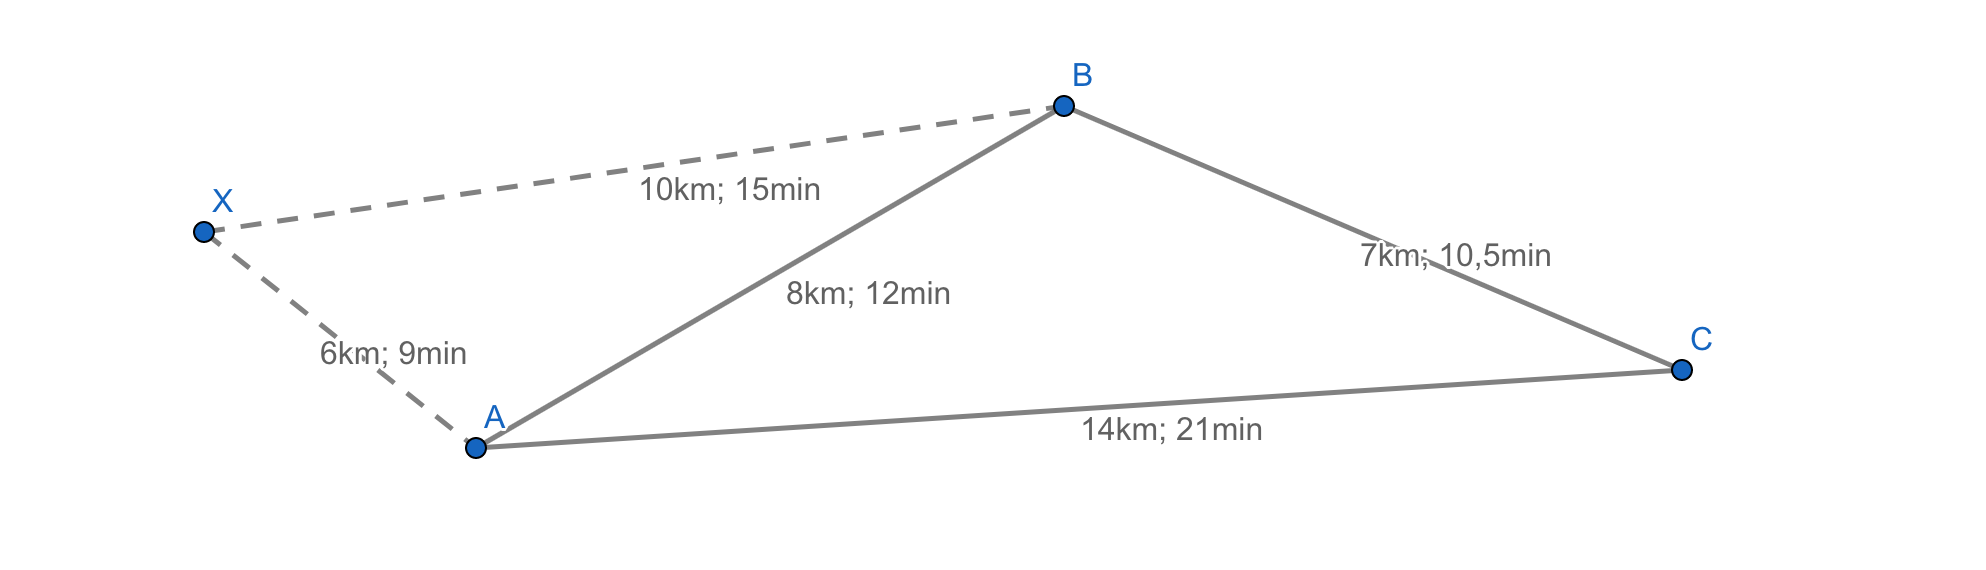
\includegraphics[width=460px]{imagen.png}

\subsection*{Anexo B}
\addcontentsline{toc}{subsection}{Anexo B}
A partir de la imagen expuesta en el Anexo A, podemos calcular cuanto le costaría a cada pasajero individualmente, y cuanto le costara a cada pasajero si comparten el viaje.

$$Q=200$$
$$V_{t}=80$$
$$P_{Km}=132,825$$
$$Costos\, \, marginales = \frac{P_{Km}}{1+g}=88,55$$
$$\overline{E}=1800$$
$$\overline{G}=400$$
$$U=0,2$$

$$T_{XA}=200+(80 \times 9)+(88,55 \times 6)=1451,3$$
$$P_{AC}=((1451,3+1800+80\times 21 + 132,825 \times 14)\times 1,2)\times \frac{100}{81}=\$10.060$$
$$P_{BC}=((2285,5+400+80\times 10,5 + 132,825 \times 7)\times 1,2)\times \frac{100}{81}=\$6.600$$
$$P_{AB}=((1451,3+80\times 12 + 132,825 \times 8)\times 1,2)\times \frac{100}{81}=\$5.146$$

$$T_{1}=10.060-(\frac{10.060}{10.060+6.600})\times (10.060-5.146)=\$7.092$$

$$T_{1}=6.600-(\frac{6.600}{10.060+6.600})\times (10.060-5.146)=\$4.653$$

Basándonos en los resultados, se puede apreciar que si hubiesen viajado normalmente desde A a B y de B a C hubiese salido $5146$ y $6600$ respectivamente, pero con nuestro modelo se distribuyeron los precios de manera justa, ambos pasajeros ahorraron dinero, y la ganancia de la compañía se mantuvo, todo gracias a que dividimos los precios en base a la razón expresada en el modelo.

Todos los valores utilizados para la ejemplificación pueden ser extraídos de las referencias.



%-------------------------------------------------------------------------------
% REFERENCIAS
%-------------------------------------------------------------------------------
\newpage
\section*{Referencias}
\addcontentsline{toc}{section}{Referencias}

<\url{https://www2.kia.cl/servicio-al-cliente/mantenimiento}>
\newline
\newline

<\url{https://cabify.com/chile/santiago/tariff-table}> 
\newline
\newline

<\url{https://www.uber.com/es-CL/blog/cambio-tarifa-scl/}>
\newline
\newline


<\url{https://www.pruebaderuta.com/cuanto-dura-un-coche.php}>
\newline
\newline

<\url{https://www.autocosmos.cl/catalogo/2018/kia/morning/10l-lx-abs/165313}>
\newline
\newline

<\url{https://www.autocosmos.cl/catalogo/2018/kia/morning/10l-lx-abs/165313}>
\newline
\newline



\end{document}

%-------------------------------------------------------------------------------
% SNIPPETS
%-------------------------------------------------------------------------------

%\begin{figure}[!ht]
%	\centering
%	\includegraphics[width=0.8\textwidth]{file_name}
%	\caption{}
%	\centering
%	\label{label:file_name}
%\end{figure}

%\begin{figure}[!ht]
%	\centering
%	\includegraphics[width=0.8\textwidth]{graph}
%	\caption{Blood pressure ranges and associated level of hypertension (American Heart Association, 2013).}
%	\centering
%	\label{label:graph}
%\end{figure}

%\begin{wrapfigure}{r}{0.30\textwidth}
%	\vspace{-40pt}
%	\begin{center}
%		\includegraphics[width=0.29\textwidth]{file_name}
%	\end{center}
%	\vspace{-20pt}
%	\caption{}
%	\label{label:file_name}
%\end{wrapfigure}

%\begin{wrapfigure}{r}{0.45\textwidth}
%	\begin{center}
%		\includegraphics[width=0.29\textwidth]{manometer}
%	\end{center}
%	\caption{Aneroid sphygmomanometer with stethoscope (Medicalexpo, 2012).}
%	\label{label:manometer}
%\end{wrapfigure}

%\begin{table}[!ht]\footnotesize
%	\centering
%	\begin{tabular}{cccccc}
%	\toprule
%	\multicolumn{2}{c} {Pearson's correlation test} & \multicolumn{4}{c} {Independent t-test} \\
%	\midrule	
%	\multicolumn{2}{c} {Gender} & \multicolumn{2}{c} {Activity level} & \multicolumn{2}{c} {Gender} \\
%	\midrule
%	Males & Females & 1st level & 6th level & Males & Females \\
%	\midrule
%	\multicolumn{2}{c} {BMI vs. SP} & \multicolumn{2}{c} {Systolic pressure} & \multicolumn{2}{c} {Systolic Pressure} \\
%	\multicolumn{2}{c} {BMI vs. DP} & \multicolumn{2}{c} {Diastolic pressure} & \multicolumn{2}{c} {Diastolic pressure} \\
%	\multicolumn{2}{c} {BMI vs. MAP} & \multicolumn{2}{c} {MAP} & \multicolumn{2}{c} {MAP} \\
%	\multicolumn{2}{c} {W:H ratio vs. SP} & \multicolumn{2}{c} {BMI} & \multicolumn{2}{c} {BMI} \\
%	\multicolumn{2}{c} {W:H ratio vs. DP} & \multicolumn{2}{c} {W:H ratio} & \multicolumn{2}{c} {W:H ratio} \\
%	\multicolumn{2}{c} {W:H ratio vs. MAP} & \multicolumn{2}{c} {\% Body fat} & \multicolumn{2}{c} {\% Body fat} \\
%	\multicolumn{2}{c} {} & \multicolumn{2}{c} {Height} & \multicolumn{2}{c} {Height} \\
%	\multicolumn{2}{c} {} & \multicolumn{2}{c} {Weight} & \multicolumn{2}{c} {Weight} \\
%	\multicolumn{2}{c} {} & \multicolumn{2}{c} {Heart rate} & \multicolumn{2}{c} {Heart rate} \\
%	\bottomrule
%	\end{tabular}
%	\caption{Parameters that were analysed and related statistical test performed for current study. BMI - body mass index; SP - systolic pressure; DP - diastolic pressure; MAP - mean arterial pressure; W:H ratio - waist to hip ratio.}
%	\label{label:tests}
%\end{table}